\documentclass{ctexart}

\title{\Large 编码器和译码器\\{\large 实验报告}}
\author{\large  信息科学技术学院 \quad 吴海\MyFont{垚} PB22051035 \\\large  信息科学技术学院 \quad 李\quad 毅 PB22051031 \\{教室:电四楼112室\quad 座位号:12}}
\date{2023年3月11日}
\usepackage{ctex}
\setCJKfamilyfont{myfont}{SimSun.ttf}
\newcommand{\MyFont}{\CJKfamily{myfont}}
\usepackage{amsmath}
\usepackage{amsfonts}
\usepackage{amssymb}
\usepackage{bm}
\usepackage{enumerate}
\usepackage{geometry}
\geometry{left=2.5cm,right=2.5cm,top=2cm,bottom=2cm}
\usepackage{fancyhdr}
\usepackage{lastpage}
\usepackage{booktabs}
\pagestyle{fancy}
\fancyhead[l]{ }
\fancyhead[r]{ }
\fancyhead[C]{
	\begin{tabular}{cclclc}
         & \multicolumn{4}{c}{\textbf{门电路测试与应用\quad 实验报告}}                                    &            \\
信息科学技术学院 & \multicolumn{2}{c}{PB22051035 吴海\MyFont{垚}} & \multicolumn{2}{c}{PB22051031 李毅} & 2024年3月11日
\end{tabular}
}
\fancyfoot[C]{ 第 {\thepage} 页,共 \pageref{LastPage} 页}
\renewcommand{\headrulewidth}{2pt}
\usepackage{graphicx}
\usepackage{geometry}
\usepackage[hidelinks]{hyperref}
\usepackage{multicol}
\usepackage{multirow}
\usepackage{ragged2e}
\usepackage[square,comma,numbers,super]{natbib}
\bibliographystyle{unsrt}
\usepackage{siunitx}
\usepackage{subfigure}
\usepackage{wrapfig}
\usepackage{xcolor}
\usepackage{cite}
\begin{document}
    \maketitle
    \thispagestyle{empty}
    
    \newpage 
    \setcounter{page}{1}

    \section*{第一部分 \quad 实验目的}
    \begin{enumerate}
        \item 掌握用逻辑门实现编码器的方法
        \item 掌握中规模集成电路编码器和译码器的工作原理以及逻辑功能
        \item 掌握74LS138用作数据分配器的方法
        \item 熟悉编码器和译码器的级联方法
        \item 能够用译码器进行组合逻辑电路设计
    \end{enumerate}
    \section*{第二部分 \quad 实验原理}
    \subsection*{1.编码器}
    在二值逻辑电路中,信号都是以高、低电平的形式给出的。因此编码器的功能就是把每一个高、低电平信号编程一个对应的二进制编码。
    \subsection*{(1)普通编码器}
    用n位二进制代码对$2^n$个信号进行编码的电路称为二进制编码器。普通编码器不允许同时输入两个以上的编码信号的编码器。
    \subsection*{(2)8线-3线优先编码器74HC148/74LS148}
    识别信号的优先级并进行编码的逻辑部件称为优先编码器。编码器74HC148的作用是将输入$I_0'-I_7'$8个状态分别编成二进制码输出,他的逻辑框图如下图所示。他有8个输入端,3个输出端,输入使能端S',输出使能端$Y'_S$和优先编码工作状态标志$Y'_{EX}$。8个输入端的优先级从$I_7'-I_0'$递减。

    可总结得出:
    \begin{enumerate}[(1)]
        \item S'=0允许编码,S'=1禁止编码,输出$Y'_2Y'_1Y'_0$=111;
        \item $Y'_S$主要用在多个编码器电路的级联控制,即$Y'_S$总是接在优先级别低得相邻编码器的S’端,当优先级别高的编码器允许编码而无输入端申请时,$Y'_S$=0,从而允许优先级别低的相邻编码器工作,反之若有优先级别高的编码器有编码时,$Y'_S$=1,禁止相邻级别低的编码器工作;
        \item $Y'_{EX}$=0表示$Y'_2Y'_1Y'_0$是编码器输出,$Y'_{EX}$=1表示$Y'_2Y'_1Y'_0$不是编码器输出
    \end{enumerate}
    \begin{minipage}[c]{0.5\textwidth}
        \centering
        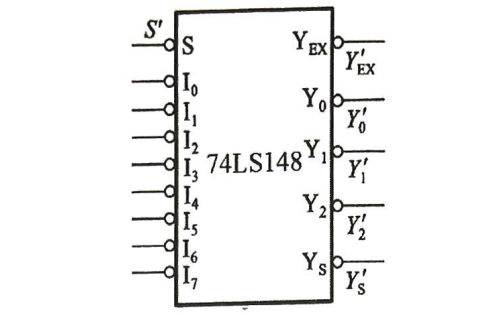
\includegraphics[width=0.8\linewidth]{2.1.1.png} 
    \end{minipage}
    \begin{minipage}[c]{0.45\textwidth}
        \centering
        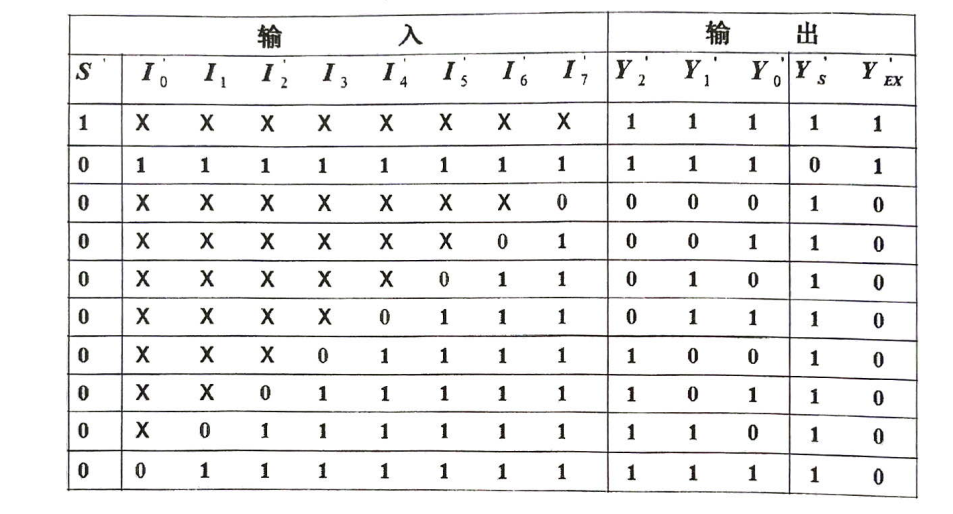
\includegraphics[width=1.2\linewidth]{2.1.2.png} 
    \end{minipage}
    
    \subsection*{2.译码器}
    译码是编码的逆过程,他的功能是将有特定含义的二进制码进行辨别,并转换成控制信号,具有译码功能的逻辑电路称为译码器。其有广泛应用,不仅限于代码的转换,终端的数字显示,还用于数据分配,存储器寻址和组合控制信号等。
    \subsection*{(1)二进制译码器}
    二进制译码器具有n个地址输入端,$2^n$个输出端和若干个控制输入端。在控制输入端为有效电平时对应每一组输入代码,只有其中一个输出端为有效电平,其余输出端则为非有效电平。每一个输出所代表的函数对应于n个输入变量的最小项。带控制输入端的译码器又是一个完整得数据分配器,若利用控制输入端中的一个作为数据输入端,则器件就成为一个数据分配器。

    以三线-八线译码器74HC138/74LS138为例进行分析:
    
    功能表如下所示,输出低电平有限效。$S_1$,$S'_2$,$S'_3$为控制输入端,当$S_1$$S'_2$$S'_3$=100时译码器工作,否则被禁止,输出全被封锁在高电平。
    
    \begin{minipage}[c]{0.5\textwidth}
        \centering
        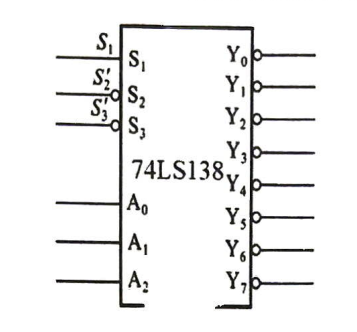
\includegraphics[width=0.8\linewidth]{2.2.1.png} 
    \end{minipage}
    \begin{minipage}[c]{0.45\textwidth}
        \centering
        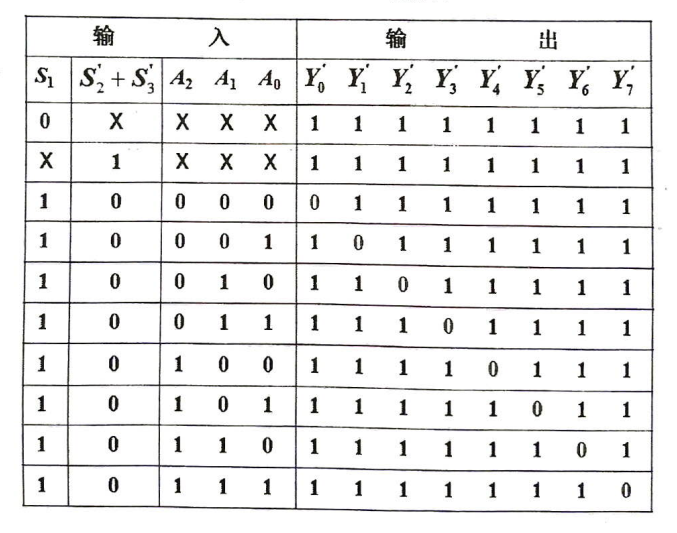
\includegraphics[width=1.2\linewidth]{2.2.2.png} 
    \end{minipage}

    \subsection*{(2)显示译码器}
    数字显示电路常由译码器,驱动器,和显示器等部分组成,本实验用CC4511,他驱动共阴极LED数码管。功能表与引脚排列如下所示:

    
    其中A,B,C,D————BCD码输入端。

    a,b,c,d,e,f,g————译码输出端,输出1有效,用来驱动共阴极LED数码管

    LT'————测试输入端,当LT'=0时,译码输出全为1.

    BI'————消隐输入端,当BI'=0时,译码输出全为0

    LE—————锁定端,当LE=1时译码器处于锁定状态,译码输出保持在LE=0时的数据,LE=0时正常译码。
    
    \begin{minipage}[c]{0.5\textwidth}
        \centering
        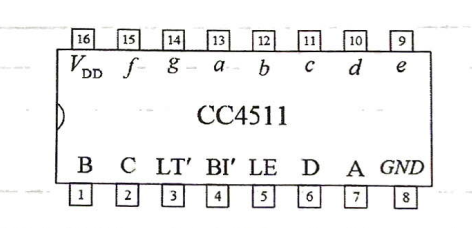
\includegraphics[width=0.8\linewidth]{2.2.3.png} 
    \end{minipage}
    \begin{minipage}[c]{0.45\textwidth}
        \centering
        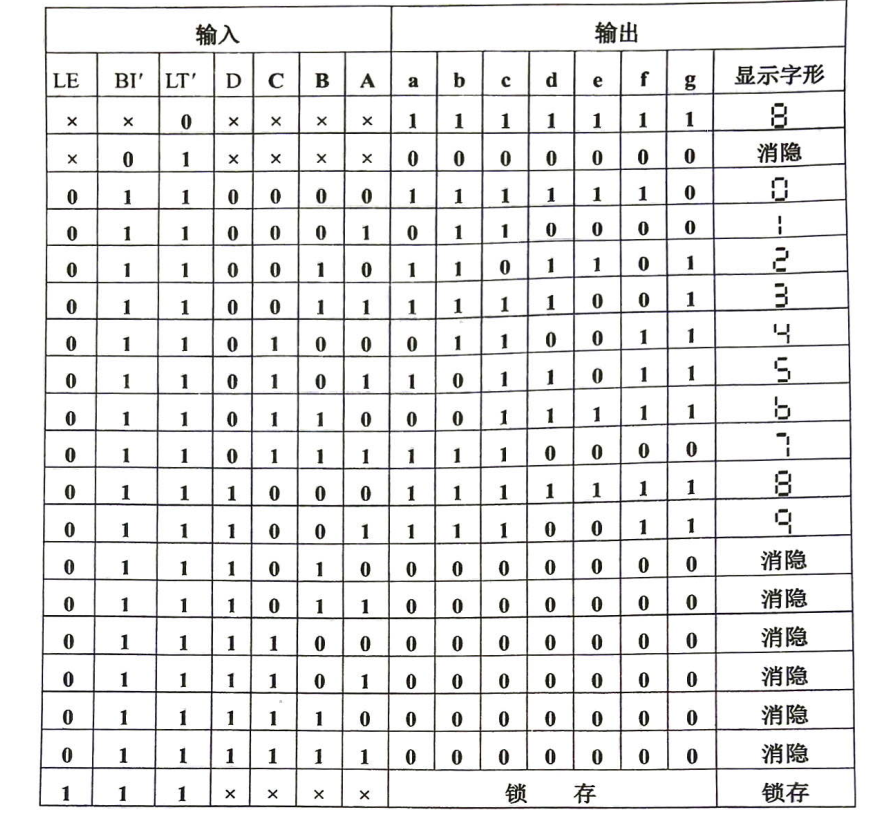
\includegraphics[width=1.2\linewidth]{2.2.4.png} 
    \end{minipage}
    \section*{第三部分 \quad 实验内容}
    \subsection*{1.用逻辑门(与非门,反相器)设计一个4线-2线的优先编码器}
    $I_0-I_3$为输入端,$Y_0-Y_1$为输出端,$Y_S$为输出使能端,$Y_{EX}$为优先编码工作标志端。

    列出逻辑真值表如下:

    \begin{table}[!ht]
    \centering 图3.1 4线-2线的优先编码器真值表
    
    \begin{tabular}{|cccc|cc|cc|}
    \hline
    $I_0$ & $I_1$ & $I_2$ & $I_3$ & $Y_0$ & $Y_1$ & $Y_S$ & $Y_{EX}$ \\ \hline
    X     & X     & X     & 1     & 1     & 1     & 0     & 1        \\ \hline
    X     & X     & 1     & 0     & 1     & 0     & 0     & 1        \\ \hline
    X     & 1     & 0     & 0     & 0     & 1     & 0     & 1        \\ \hline
    1     & 0     & 0     & 0     & 0     & 0     & 0     & 1        \\ \hline
    0     & 0     & 0     & 0     & 0     & 0     & 1     & 0        \\ \hline
    \end{tabular}
    \end{table}

    使用卡诺图化简并改写为与非-与非形式得到逻辑表达式为:

    $$Y_1=I_3+I_2I'_3=(I'_2I'_3)'$$
    $$Y_0=I_3+I_1I'_2I'_3=(I'_3(I_1I'_2I'_3)')'$$
    $$Y_S=I'_0I'_1I'_2I'_3=((I'_0I'_1I'_2I'_3)')'$$
    $$Y_{EX}=(I'_0I'_1I'_2I'_3)'$$

    画出电路图如下:

    \begin{minipage}[c]{\textwidth}
        \centering 
        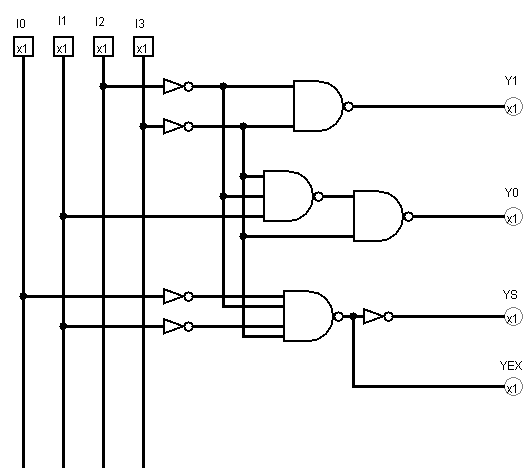
\includegraphics[width=0.75\linewidth]{3.1.png} 
        
        图3.1:4线-2线的优先编码器逻辑电路图
    \end{minipage}

    \subsection*{2.将74LS138用作数据分配器,将1Hz连续脉冲信号加到电路的控制输入端,输出接发光二级管,改变输入地址码$A_2$、$A_1$、$A_0$的值,观察实验现象,记录实验结果}

     电路图如下:

    \begin{minipage}[l]{\textwidth}
        \centering 
        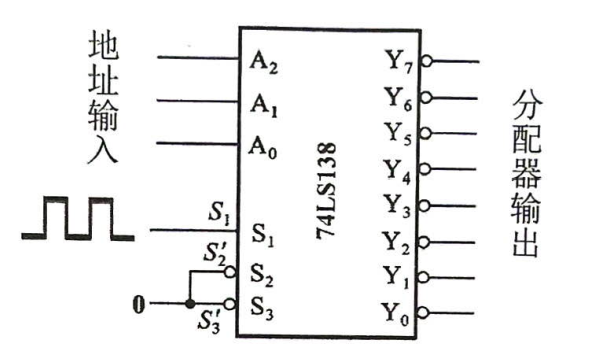
\includegraphics[width=0.7\linewidth]{3.2.png} 
        
        图3.2:74LS138作数据分配器
    \end{minipage}

    记录实验结果得到逻辑真值表如下:
\begin{table}[!ht]
\centering  表3.2:74LS138作数据分配器逻辑真值表

\begin{tabular}{|ccccc|cccccccc|}
\hline
\multicolumn{5}{|c|}{输入}                                                                 & \multicolumn{8}{c|}{输出}                                               \\ \hline
\multicolumn{1}{|c|}{$S_1$}   & \multicolumn{1}{c|}{$S'_2+S'_3$} & $A_2$ & $A_1$ & $A_0$ & $Y'_0$ & $Y'_1$ & $Y'_2$ & $Y'_3$ & $Y'_4$ & $Y'_5$ & $Y'_6$ & $Y'_7$ \\ \hline
\multicolumn{1}{|c|}{0}       & \multicolumn{1}{c|}{x}           & x     & x     & x     & 1      & 1      & 1      & 1      & 1      & 1      & 1      & 1      \\ \hline
\multicolumn{1}{|c|}{x}       & \multicolumn{1}{c|}{1}           & x     & x     & x     & 1      & 1      & 1      & 1      & 1      & 1      & 1      & 1      \\ \hline
\multicolumn{1}{|c|}{\_|¯|\_} & \multicolumn{1}{c|}{0}           & 0     & 0     & 0     & ¯|\_|¯ & 1      & 1      & 1      & 1      & 1      & 1      & 1      \\ \hline
\multicolumn{1}{|c|}{\_|¯|\_} & \multicolumn{1}{c|}{0}           & 0     & 0     & 1     & 1      & ¯|\_|¯ & 1      & 1      & 1      & 1      & 1      & 1      \\ \hline
\multicolumn{1}{|c|}{\_|¯|\_} & \multicolumn{1}{c|}{0}           & 0     & 1     & 0     & 1      & 1      & ¯|\_|¯ & 1      & 1      & 1      & 1      & 1      \\ \hline
\multicolumn{1}{|c|}{\_|¯|\_} & \multicolumn{1}{c|}{0}           & 0     & 1     & 1     & 1      & 1      & 1      & ¯|\_|¯ & 1      & 1      & 1      & 1      \\ \hline
\multicolumn{1}{|c|}{\_|¯|\_} & \multicolumn{1}{c|}{0}           & 1     & 0     & 0     & 1      & 1      & 1      & 1      & ¯|\_|¯ & 1      & 1      & 1      \\ \hline
\multicolumn{1}{|c|}{\_|¯|\_} & \multicolumn{1}{c|}{0}           & 1     & 0     & 1     & 1      & 1      & 1      & 1      & 1      & ¯|\_|¯ & 1      & 1    \\ \hline
\multicolumn{1}{|c|}{\_|¯|\_} & \multicolumn{1}{c|}{0}           & 1     & 1     & 0     & 1      & 1      & 1      & 1      & 1      & 1      & ¯|\_|¯ & 1      \\ \hline
\multicolumn{1}{|c|}{\_|¯|\_} & \multicolumn{1}{c|}{0}           & 1     & 1     & 1     & 1      & 1      & 1      & 1      & 1      & 1      & 1      & ¯|\_|¯ \\ \hline
\end{tabular}
\end{table}

\subsection*{3.验证编码器74LS148和译码器74LS138的逻辑功能}
电路连接如图3.3所示:

    \begin{minipage}[l]{\textwidth}
        \centering 
        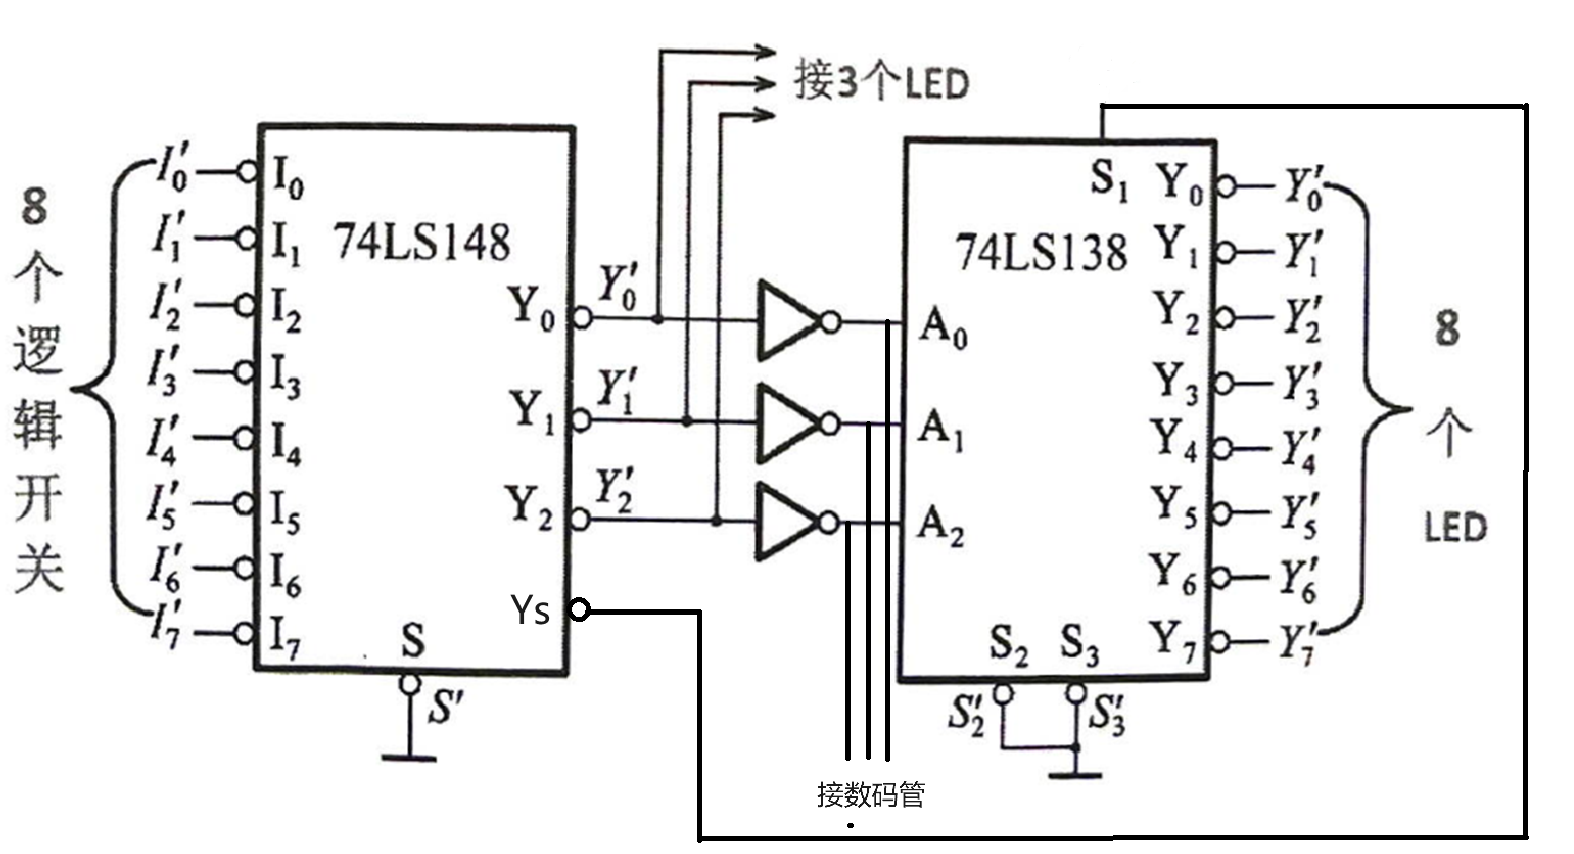
\includegraphics[width=\linewidth]{3.3.png} 
        
        图3.3:验证编码器74LS148和译码器74LS138的逻辑功能
    \end{minipage}

输出状态记录表3.3所示

\begin{table}[!ht]
\centering 表3.3 编码器74LS148和译码器74LS138的输出状态

\begin{tabular}{|cccccccc|ccc|ccc|cccccccc|}
\hline
\multicolumn{11}{|c|}{74LS148(编码器)} & \multicolumn{11}{c|}{74LS138(译码器)}       \\ \hline
$I'_0$ & $I'_1$ & $I'_2$ & $I'_3$ & $I'_4$ & $I'_5$ & $I'_6$ & $I'_7$ & $Y'_2$ & $Y'_1$ & $Y'_0$ & $A_2$ & $A_1$ & $A_0$ & $Y'_0$ & $Y'_1$ & $Y'_2$ & $Y'_3$ & $Y'_4$ & $Y'_5$ & $Y'_6$ & $Y'_7$ \\ \hline
1      & 1      & 1      & 1      & 1      & 1      & 1      & 1      & 1      & 1      & 1      & 0     & 0     & 0     & 1      & 1      & 1      & 1      & 1      & 1      & 1      & 1      \\ \hline
0      & 1      & 1      & 1      & 1      & 1      & 1      & 1      & 1      & 1      & 1      & 0     & 0     & 0     & 0      & 1      & 1      & 1      & 1      & 1      & 1      & 1      \\ \hline
x      & 0      & 1      & 1      & 1      & 1      & 1      & 1      & 1      & 1      & 0      & 0     & 0     & 1     & 1      & 0      & 1      & 1      & 1      & 1      & 1      & 1      \\ \hline
x      & x      & 0      & 1      & 1      & 1      & 1      & 1      & 1      & 0      & 1      & 0     & 1     & 0     & 1      & 1      & 0      & 1      & 1      & 1      & 1      & 1      \\ \hline
x      & x      & x      & 0      & 1      & 1      & 1      & 1      & 1      & 0      & 0      & 0     & 1     & 1     & 1      & 1      & 1      & 0      & 1      & 1      & 1      & 1      \\ \hline
x      & x      & x      & x      & 0      & 1      & 1      & 1      & 0      & 1      & 1      & 1     & 0     & 0     & 1      & 1      & 1      & 1      & 0      & 1      & 1      & 1      \\ \hline
x      & x      & x      & x      & x      & 0      & 1      & 1      & 0      & 1      & 0      & 1     & 0     & 1     & 1      & 1      & 1      & 1      & 1      & 0      & 1      & 1      \\ \hline
x      & x      & x      & x      & x      & x      & 0      & 1      & 0      & 0      & 1      & 1     & 1     & 0     & 1      & 1      & 1      & 1      & 1      & 1      & 0      & 1      \\ \hline
x      & x      & x      & x      & x      & x      & x      & 0      & 0      & 0      & 0      & 1     & 1     & 1     & 1      & 1      & 1      & 1      & 1      & 1      & 1      & 0      \\ \hline
\end{tabular}
\end{table}

\newpage
\subsection*{4.设计一个具有3路报警信号的报警装置}
当第一路有报警信号时,数码管显示“1”,当第二路有信号时,数码管显示“2”,当第三路有信号时,数码管显示“3”;当有两路或两路以上有报警信号时,数码管显示“8”,无报警信号时,数码管显示“0”。

使用74LS138译码器实现电路。使用$Y_1$,$Y_2$,$Y_3$代表1,2,3路报警信号的输入,接$A_2$,$A_1$,$A_0$得到对应的最小项。根据数码管CC4511的功能表得出逻辑表达式为:

$$A=m(1,4)$$
$$B=m(2,4)$$
$$C=0$$
$$D=m(3,5,6,7)$$

画出电路图如下:

    \begin{minipage}[l]{\textwidth}
        \centering 
        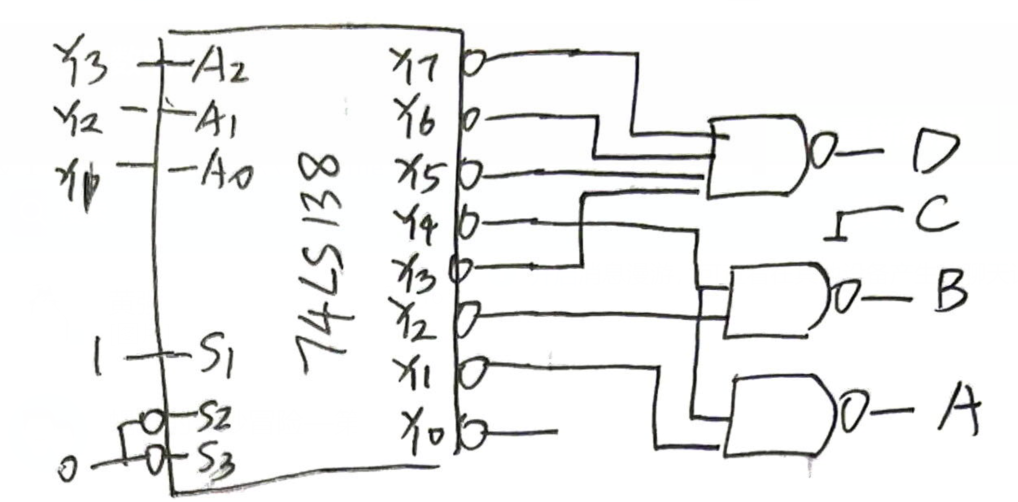
\includegraphics[width=\linewidth]{3.4.png} 
        
        图3.4:3路报警信号的报警装置电路图
    \end{minipage}

\subsection*{5.试用两片74LS138和74LS20双与非门设计下面的多输出函数,画出逻辑电路图。}

将两片74LS138连接成4线-16线译码器,A接两片74LS138的$A_0$端,B接两片74LS138的$A_1$端,C接两片74LS138的$A_2$端,D'接左边一片(对应最小项为$m_0-m_7$)74LS138的$S_1$端,D接右边一片(对应最小项为$m_8-m_15$)74LS138的$S_1$端。

要求多输出函数为:

$$Y_1=BC'$$
$$Y_2=AB'CD+A'BC+AB'D$$
化为最小项形式为:
$$Y_1=m(2,3,10,11)$$
$$Y_2=m(6,9,13,14)$$

画出电路图如下:

    \begin{minipage}[l]{\textwidth}
        \centering 
        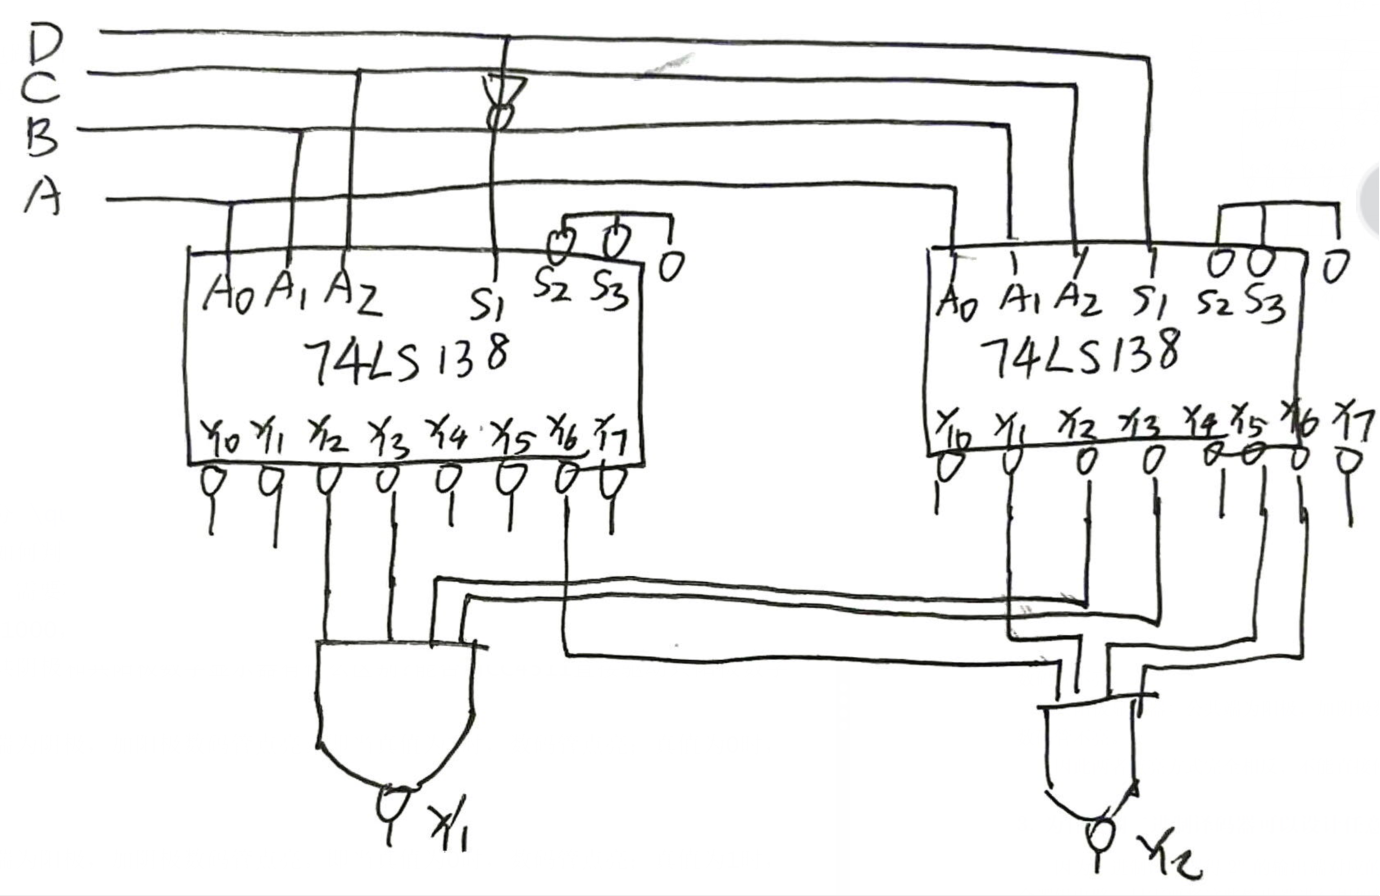
\includegraphics[width=\linewidth]{3.5.png} 
        
        图3.5:指定多输出函数电路图
    \end{minipage}
    
    \section*{第四部分 \quad 思考题}
    \subsection*{1.如何判断一个数码管的好坏}
    要检查数码管的好坏,需要检查数码管各段是否都能正常工作。为了一次检验,数码管连接好电源与地后,DCBA输入1000,若可以正常显示出8即为正常。
    \subsection*{2.共阴极和共阳极数字显示器有什么区别?能否用CC4511直接驱动共阳极数字显示器}
    共阴极显示器:公共端为阴极,加阳极数码管点亮。即当真值为1时,数码管点亮;真值为0时,数码管不亮。
    
    共阳极显示器:公共端为阳极,加阴极数码管点亮。即当真值为0时,数码管点亮;真值为1时,数码管不亮。

    因此两者点亮方式完全相反,不能直接使用CC4511来驱动共阳极数字显示器,需要稍加改变,

    \subsection*{3.为什么用二进制译码器可以设计任意的组合逻辑电路}
    因为二进制译码器得$2^n$的输出端对应的就是对于n个变量的全部最小项,因此对于n个变量的组合逻辑电路,只需要将这些输出端进行相加组合即可得出响应逻辑表达式。

    \subsection*{4.总结用集成电路进行功能扩展的方法}
    因为进行功能扩展用的都是相同的集成电路,在实现相应功能上效果都一样,主要问题是具体使用时到底是用哪一个集成电路,需要用到电路的控制输入端或者是使能端,输出工作状态标志等。比如将输出的一个变量用来控制使能端来选择集成电路;上一级的输出工作状态标志输出给下一级使能端,达到不同优先级的控制。
\end{document}


